\section{Objektliste}
\thispagestyle{fancy}

Vi måtte danne oss eit bilde over alle komponentane som eksisterte og var tilkopla styresystmet. Dette for å gje oss ei o
oversikt over komponentane vi skulle styre, meg også kva \gls{IEC} blokker \ref{IEC Seksjon} vi trengde og programmere.

\begin{figure}[htbp]
    \centering
    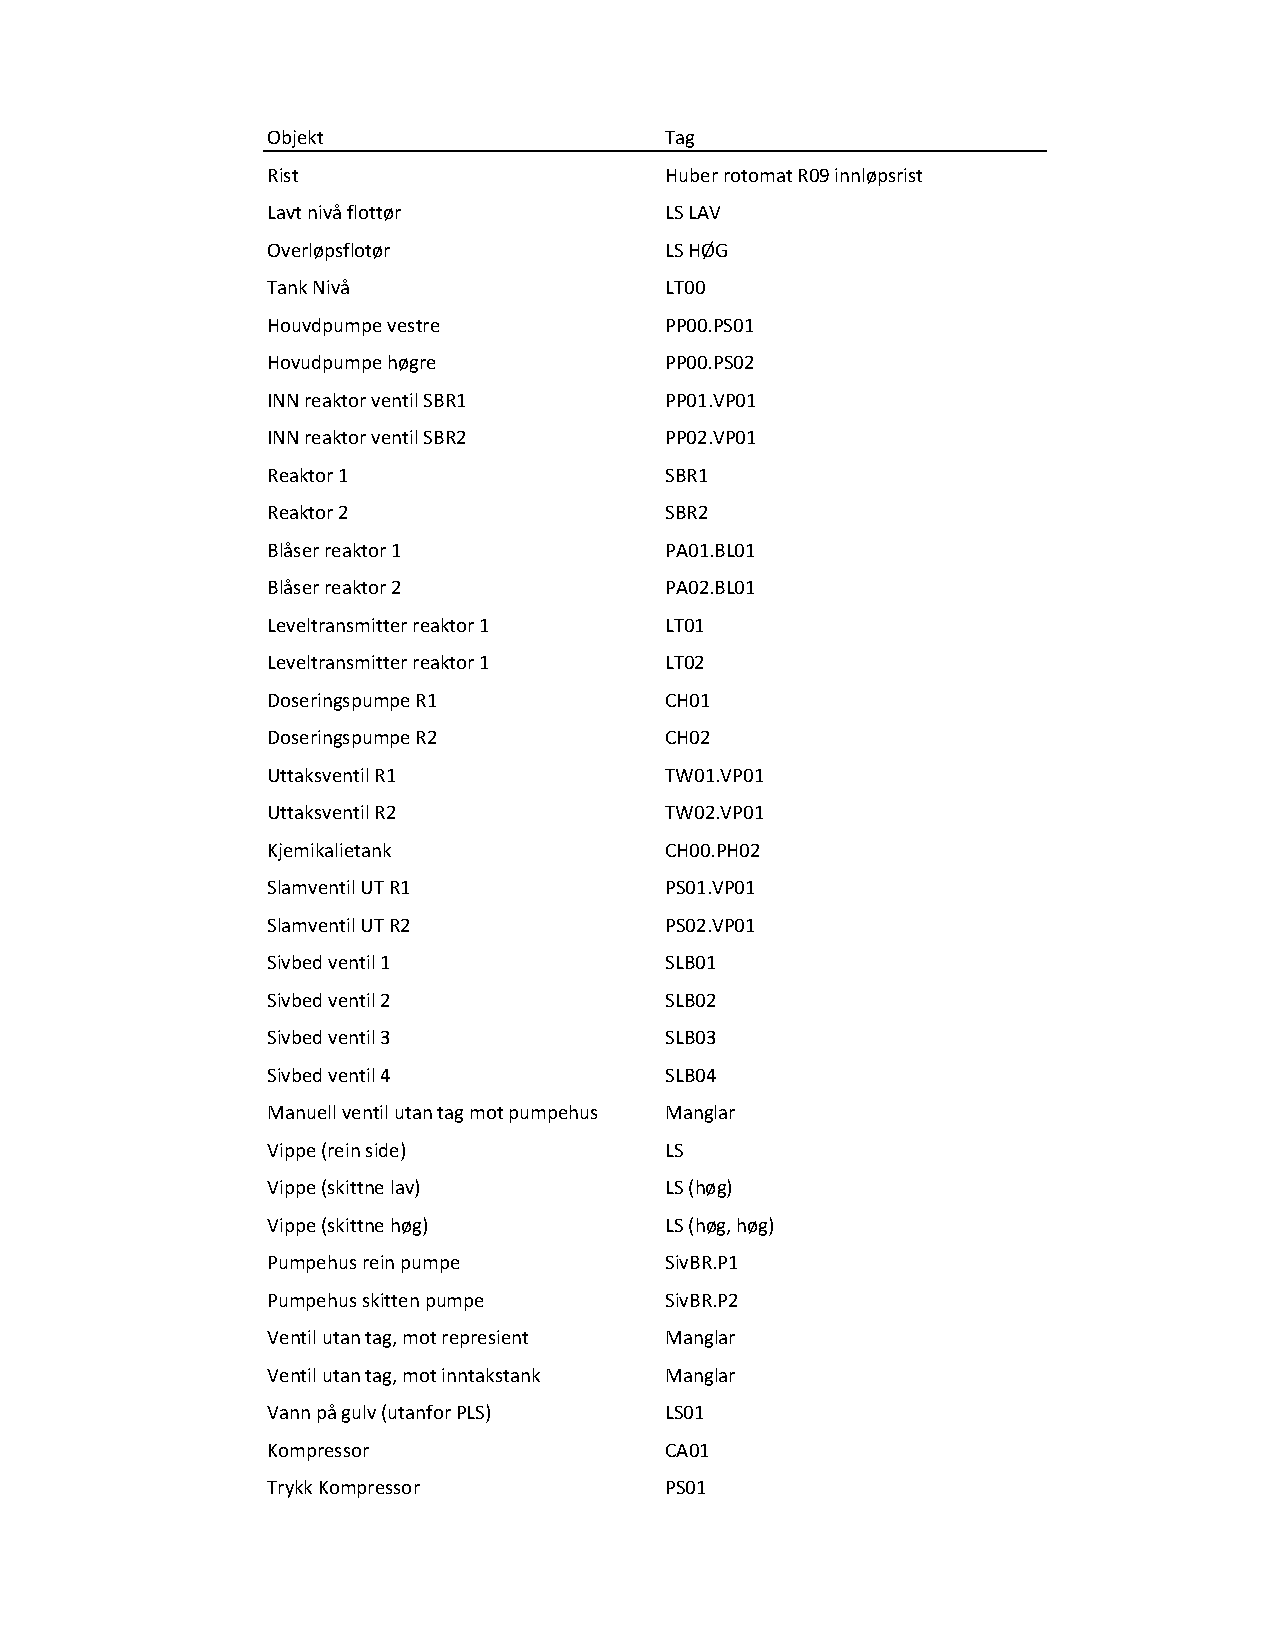
\includegraphics[scale=0.6, page=1]{Appendix/Objektliste_midlertidig.pdf}
    \caption{Objektliste}
    \label{fig:Objektliste}
\end{figure}

\newpage




% Place the PDF as a full page


% Manually add a caption on the next page or in a suitable position
\begin{tikzpicture}[remember picture, overlay]
    % Include the PDF page rotated, positioned at the center of the page
    \node[inner sep=0pt] at (current page.center) {
        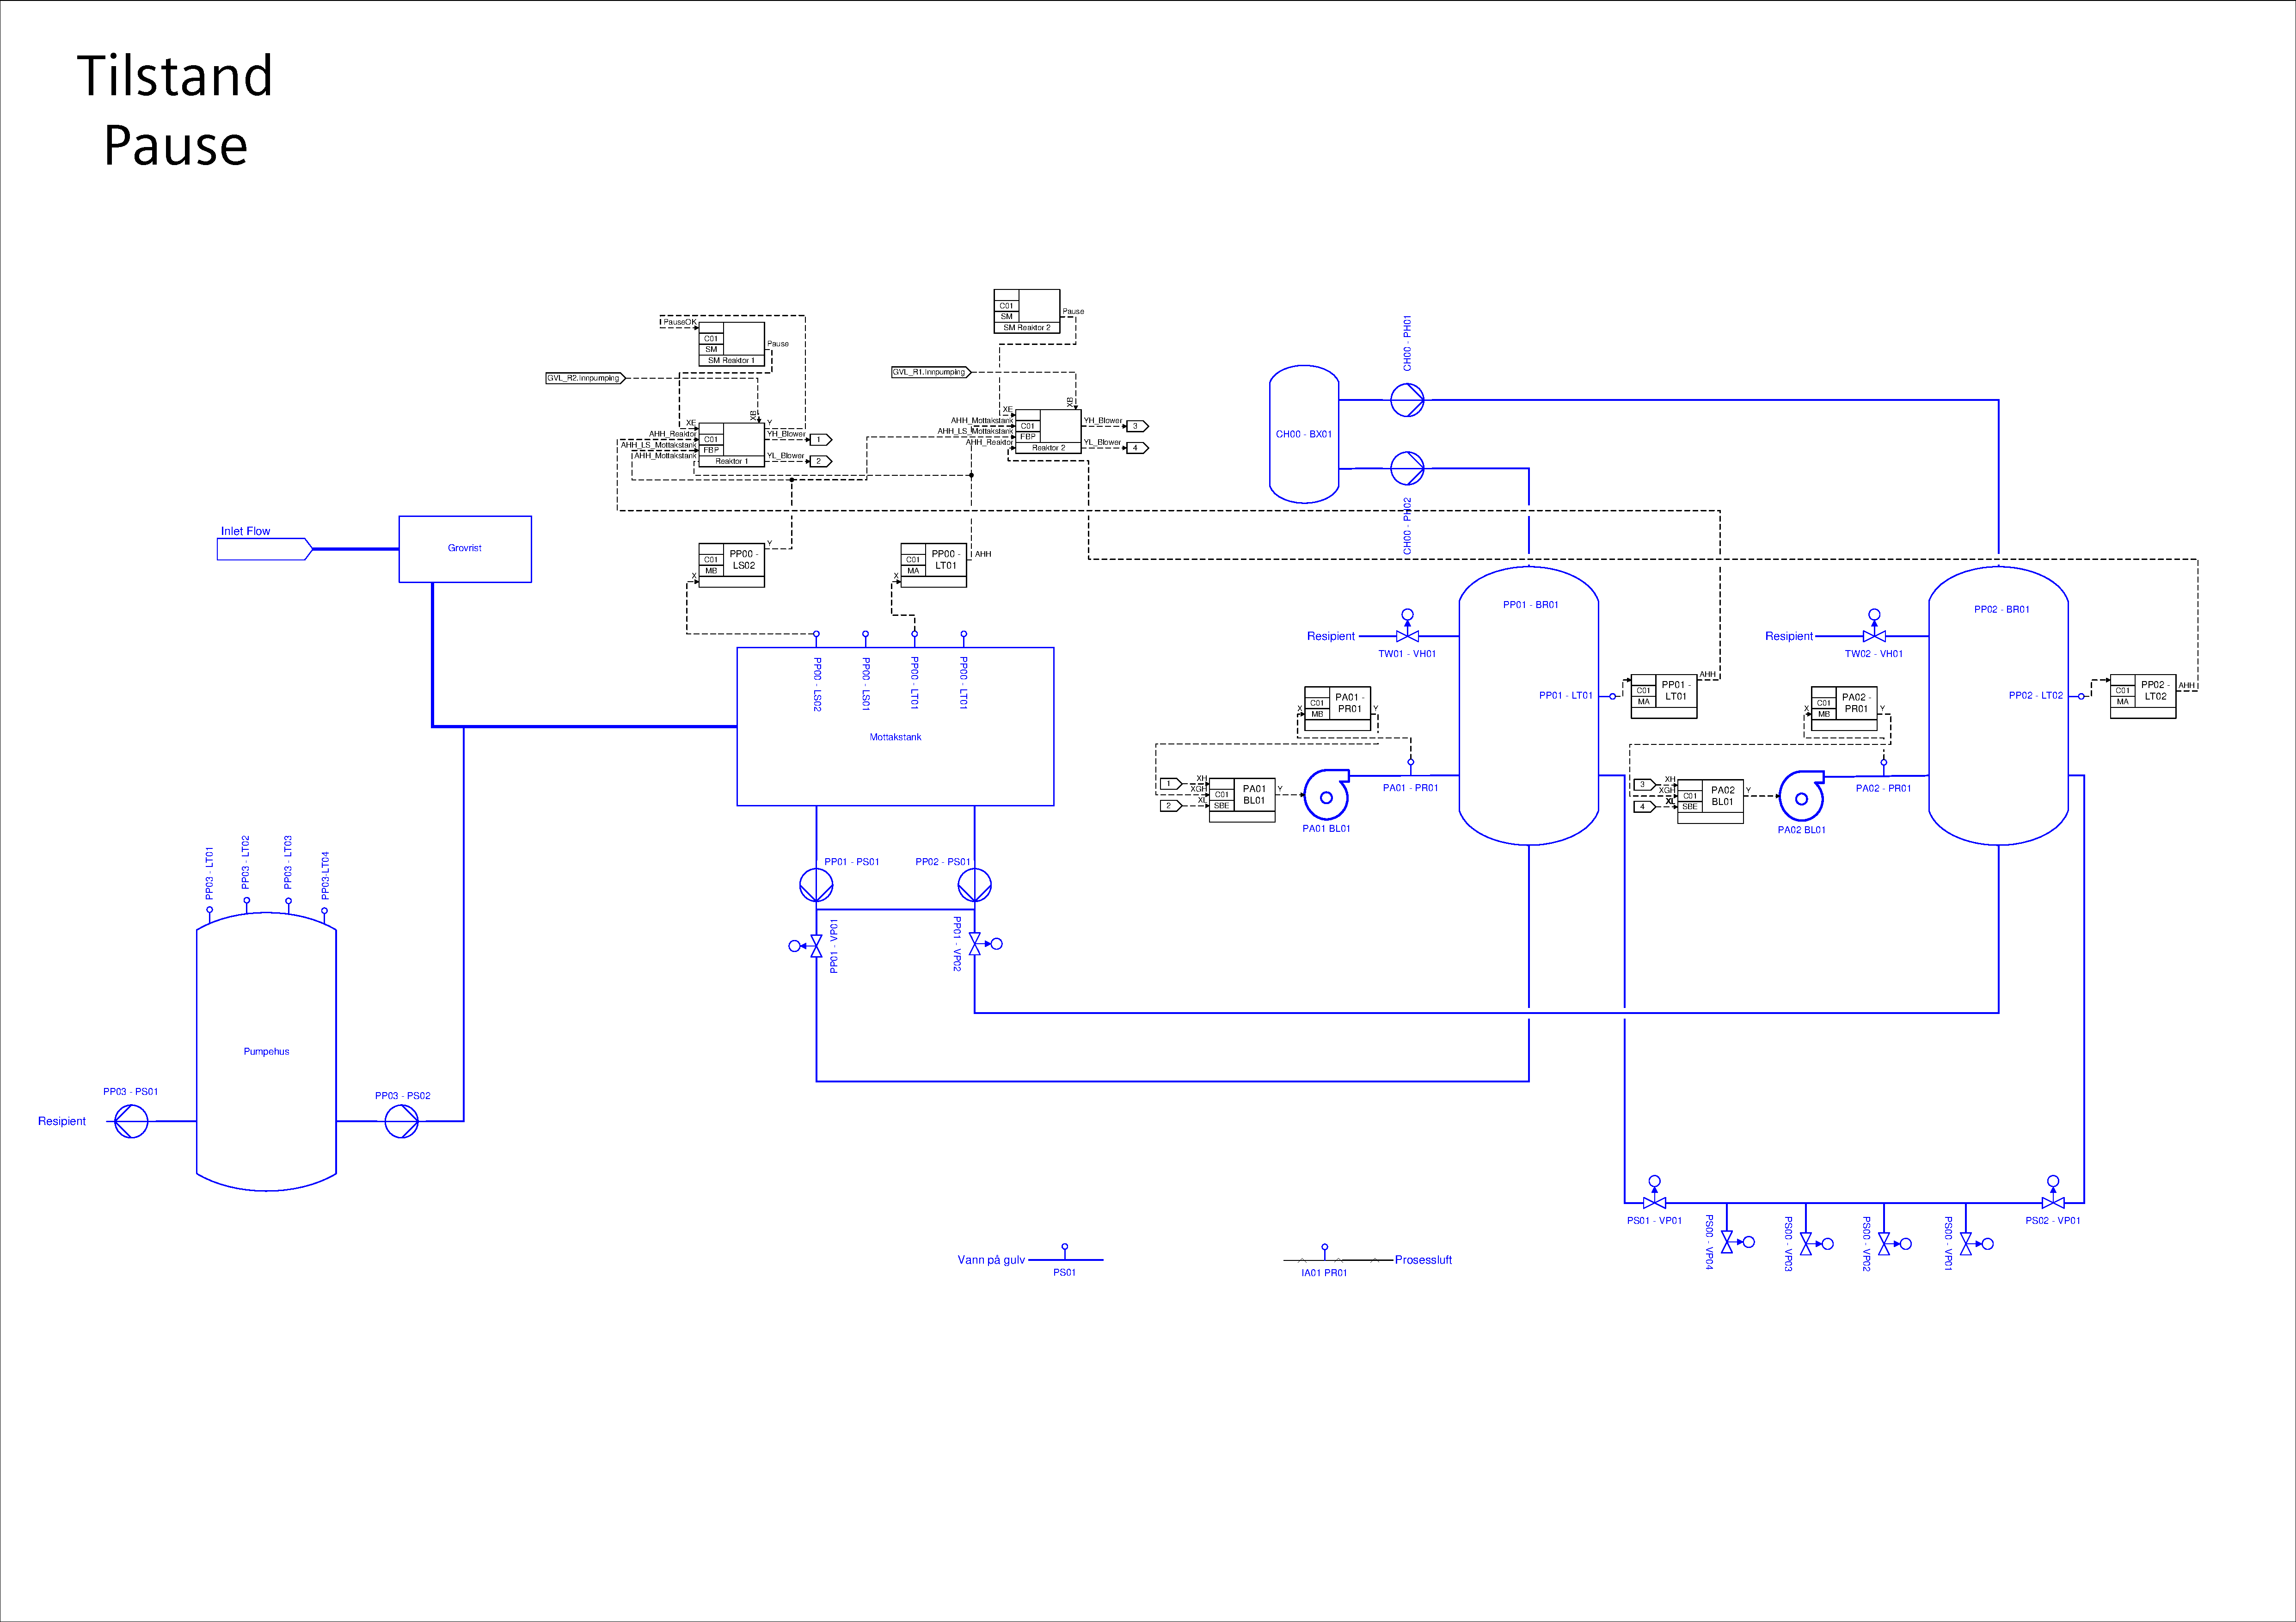
\includegraphics[angle=90, width=\paperwidth, keepaspectratio]{Bilder/SCD.pdf}
    };

    % Place the caption at the bottom of the page
    \node[anchor=south, yshift=10mm] at (current page.south) { % Adjust yshift to position the caption
        \begin{minipage}{\textwidth}
            \centering
            \captionof{figure}{SCD innpumpingssekvens}
            \label{fig:SCD}
        \end{minipage}
    };
\end{tikzpicture}


\newpage
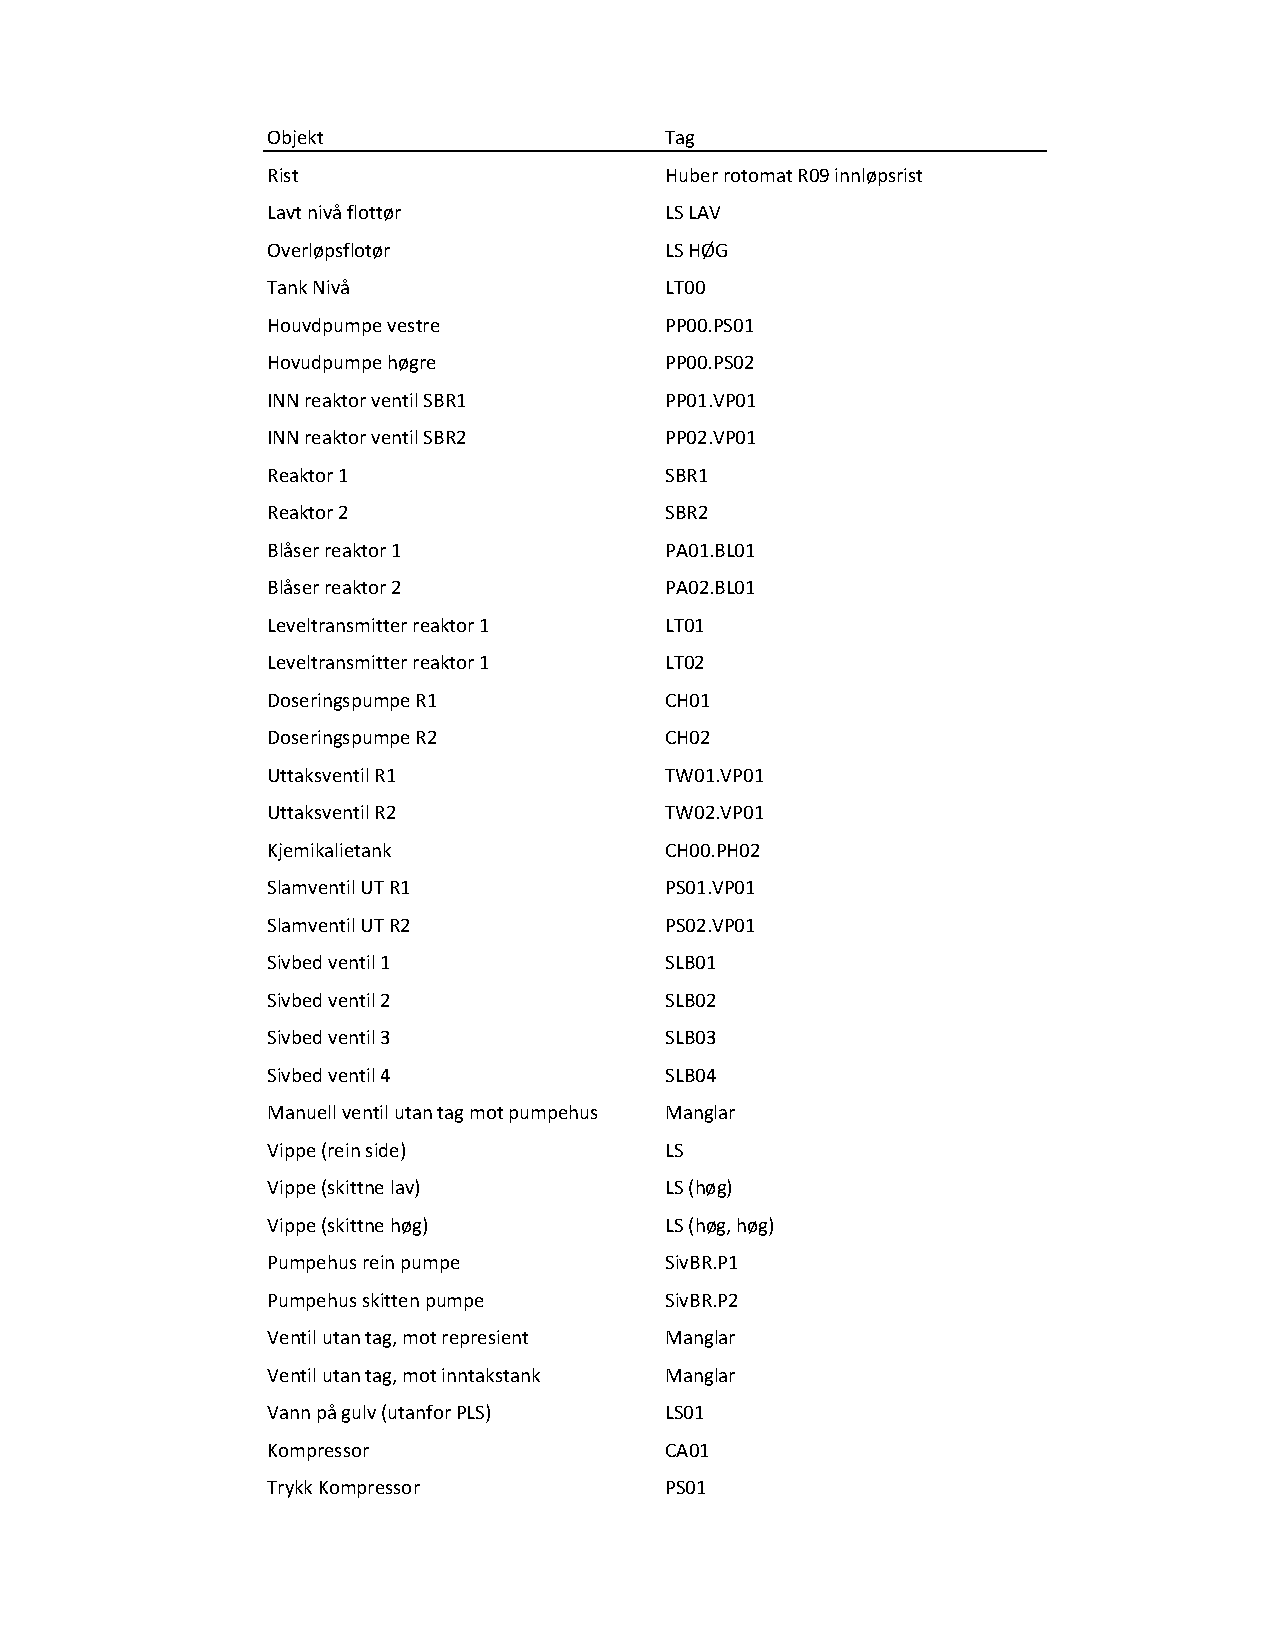
\includepdf[pages=1, scale=0.75, pagecommand={\section{Objektliste}\thispagestyle{empty}}]{Appendix/Objektliste_midlertidig.pdf}

\newpage
